% !TEX root = ../thesis.tex

\chapter{Flowcharts}

\section{Overview}
\begin{figure}[h!]
    \begin{center}
        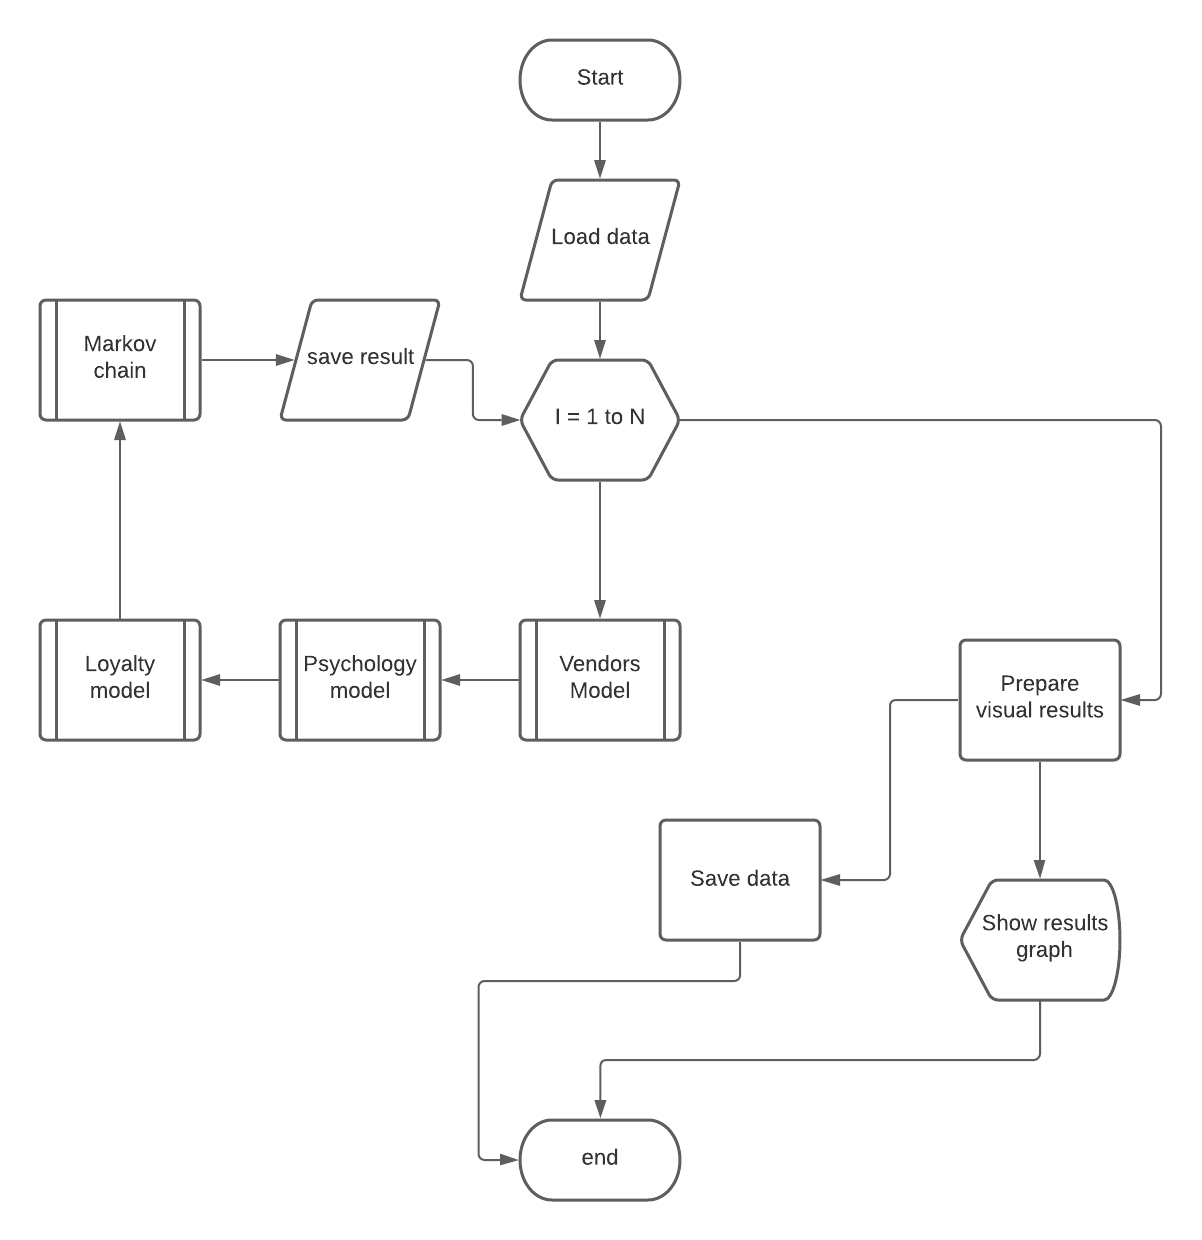
\includegraphics[width=350]{flowchart_overview}
    \end{center}
    \caption{Flowchart overview}
    \label{flowchart_overview}
\end{figure}
\newpage
\section{Vendor model}
\begin{figure}[h!]
    \begin{center}
        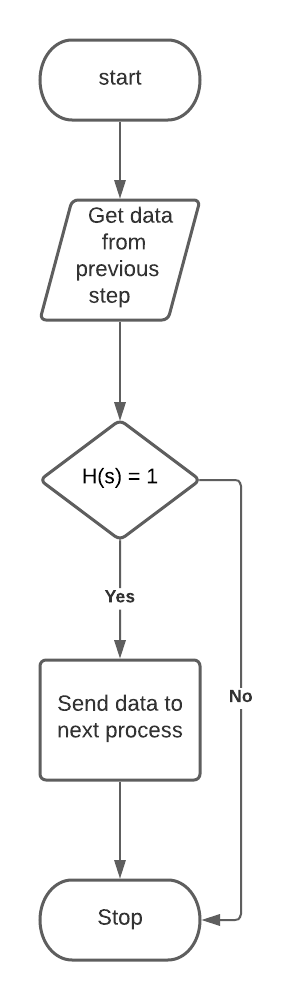
\includegraphics[width=180]{flowchart_vendor}
    \end{center}
    \caption{Flowchart vendor model}
    \label{flowchart_vendor}
\end{figure}
\section{Psychology model}
\begin{figure}[h!]
    \begin{center}
        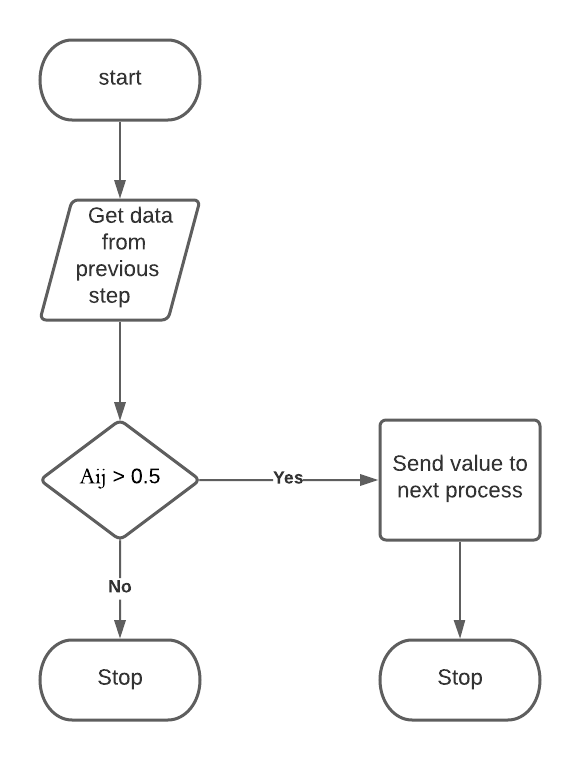
\includegraphics[width=180]{flowchart_psychology}
    \end{center}
    \caption{Flowchart psychology model}
    \label{flowchart_psychology}
\end{figure}
\newpage
\section{Loyalty model}
\begin{figure}[h!]
    \begin{center}
        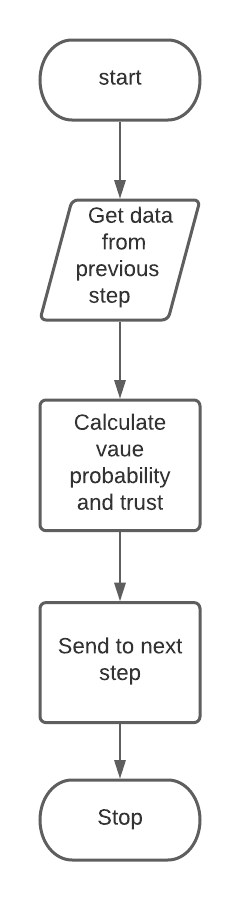
\includegraphics[width=60]{flowchart_loyalty}
    \end{center}
    \caption{Flowchart loyalty model}
    \label{flowchart_loyalty}
\end{figure}
\section{Markov hidden model}
\begin{figure}[h!]
    \begin{center}
        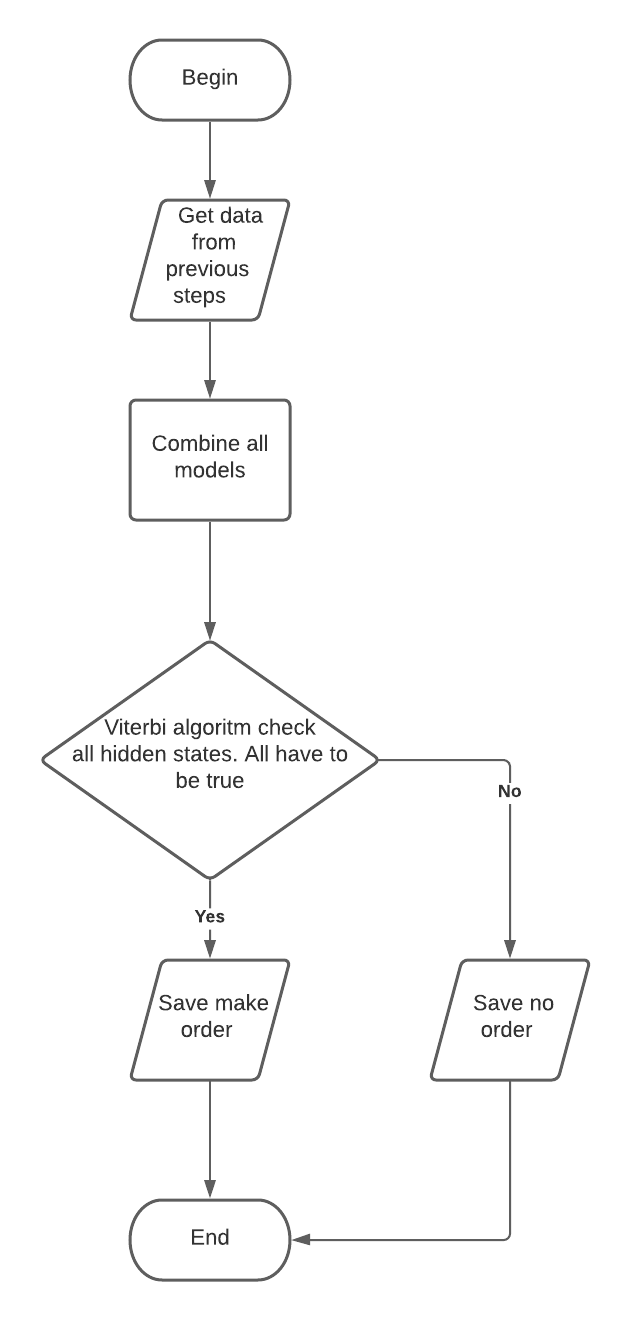
\includegraphics[width=230]{flowchart_markovpng}
    \end{center}
    \caption{Flowchart markov chain}
    \label{flowchart_markov}
\end{figure}
\newpage
